\chapter{Data Understanding and Preparation}
\label{ch:capitolo1}

\section{Data Semantics}\label{sec:data_semantics}
The dataset \textit{train.csv} contains 16431 titles of different forms of visual entertainment that have been rated on IMDb, an online database of information related to films, television series etc. 
Each record is described by 23 attributes, both numerical and non-numerical. 
All the variables of the dataset are introduced and explained in Table 1.1 and Table 1.2.
\begin{table}[h]
    \centering
    \begin{tabular}{|l|l|l|} % Using 'l' for left alignment of columns
        \hline
        \textbf{Attribute} & \textbf{Type} & \textbf{Description} \\ 
        \hline
        originalTitle & Nominal & Title in its original language \\  
        \hline
        rating & Ordinal & IMDB title rating class \\
        & & The range is from (0,1] to (9,10] \\ 
        \hline
        worstRating & Ordinal & Worst title rating \\ 
        \hline
        bestRating & Ordinal & Best title rating \\ 
        \hline
        titleType & Nominal & The format of the title \\ 
        \hline
        canHaveEpisodes & Nominal (Binary) & Whether or not the title can have episodes \\ 
        & & True: can have episodes; False: cannot have episodes \\ 
        \hline
        isRatable & Nominal (Binary) & Whether or not the title can be rated by users \\ 
        & & True: it can be rated; False: cannot be rated \\ 
        \hline
        isAdult & Nominal (Binary) & Whether or not the title is for adults \\ 
        & & 0: non-adult title; 1: adult title \\ 
        \hline
        countryOfOrigin & Nominal & The country(ies) where the title was produced \\ 
        \hline
        genres & Nominal & The genre(s) associated with the title \\ 
        \hline
    \end{tabular}
    \caption{Description of non-numerical attributes}
    \label{tab:attributes}
\end{table}
\begin{table}[h]
    \centering
    \begin{tabular}{|l|l|l|} % Using 'l' for left alignment of columns
        \hline
        \textbf{Attribute} & \textbf{Type} & \textbf{Description} \\ 
        \hline
        runtimeMinutes & Numeric & Runtime of the title expressed in minutes \\ 
        \hline
        startYear & Interval & Release/start year of a title \\ 
        \hline
        endYear & Interval & TV Series end year \\
        \hline
        awardWins & Numeric & Number of awards the title won \\ 
        \hline
        numVotes & Numeric & Number of votes the title has received \\ 
        \hline
        totalImages & Numeric & Number of Images on the IMDb title page \\ 
        \hline
        totalVideos & Numeric & Number of Videos on the IMDb title page \\ 
        \hline
        totalCredits & Numeric & Number of Credits for the title \\ 
        \hline
        criticReviewsTotal & Numeric & Total Number of Critic Reviews \\ 
        \hline
        awardNominationsExcludeWins & Numeric & Number of award nominations excluding wins \\ 
        \hline
        numRegions & Numeric & The regions number for this version of the title \\ 
        \hline
        userReviewsTotal & Numeric & Number of User Reviews \\ 
        \hline
        ratingCount & Numeric & The total number of user ratings for the title \\ 
        \hline
    \end{tabular}
    \caption{Description of numerical attributes}
    \label{tab:numerical_attributes}
\end{table}
\section{Distribution of the variables and statistics}\label{sec:variable_distrib}
This section will give an overview about the distribution of variables that has been carried on to understand patterns, detect meaningful statistics and assess their relevance to the project. 

\subsection{Discrete attributes}
\textbf{DA CAMBIARE IN BASE AI GRAFICI CHE DECIDIAMO DI TENERE}
In this paragraph, the most informative discrete attributes of the dataset are examined to provide an overview of their statistics and frequencies. \\
From Fig.1.1(a), it is observed that the classes of the \texttt{titleType} attribute are unbalanced, with \textit{movie} being the most frequent class (5535 records) and \textit{tvShort} the least frequent (40 records). 
By analyzing the \texttt{canHaveEpisodes} attribute within these \texttt{titleType} values, it is found that only \textit{tvSeries} and \textit{tvMiniSeries} can have episodes, as expected.
As shown in Fig.1.1(b), the frequency of rating classes is slighly skewed toward higher values, with the most frequent rating class being (7, 8], which is the rating of 4822 titles.
Another important aspect is that all 16341 titles are ratable and the vast majority of them (16005) are non-adults contents, as shown in Fig.1.1(c)
Finally, as indicated in Fig.1.1(d), an analysis of the \texttt{genres} variable across different \texttt{titleType} values reveals that \textit{Drama} and \textit{Comedy} are the most common genres, as they appear in the top 3 genres of nearly every \textit{titleType} category.
% \begin{figure}[h!]
%     \centering
%     \begin{subfigure}[b]{0.48\textwidth}
%         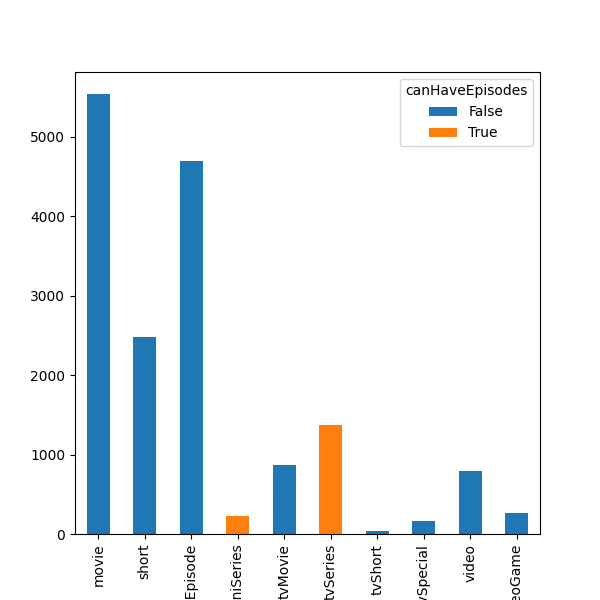
\includegraphics[width=\textwidth]{plots/fig1_a.png}
%         \caption{Counting of the title types frequencies combined with the canHaveEpisodes variable}
%         \label{fig:sub1}
%     \end{subfigure}
%     \subfigure[]{
%         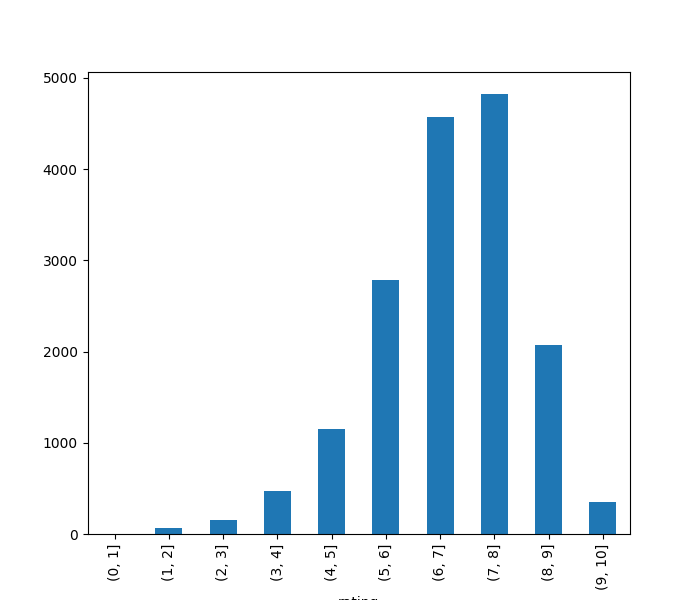
\includegraphics[width=0.48\textwidth]{plots/fig1_b.png}
%     }
%     \subfigure[]{
%         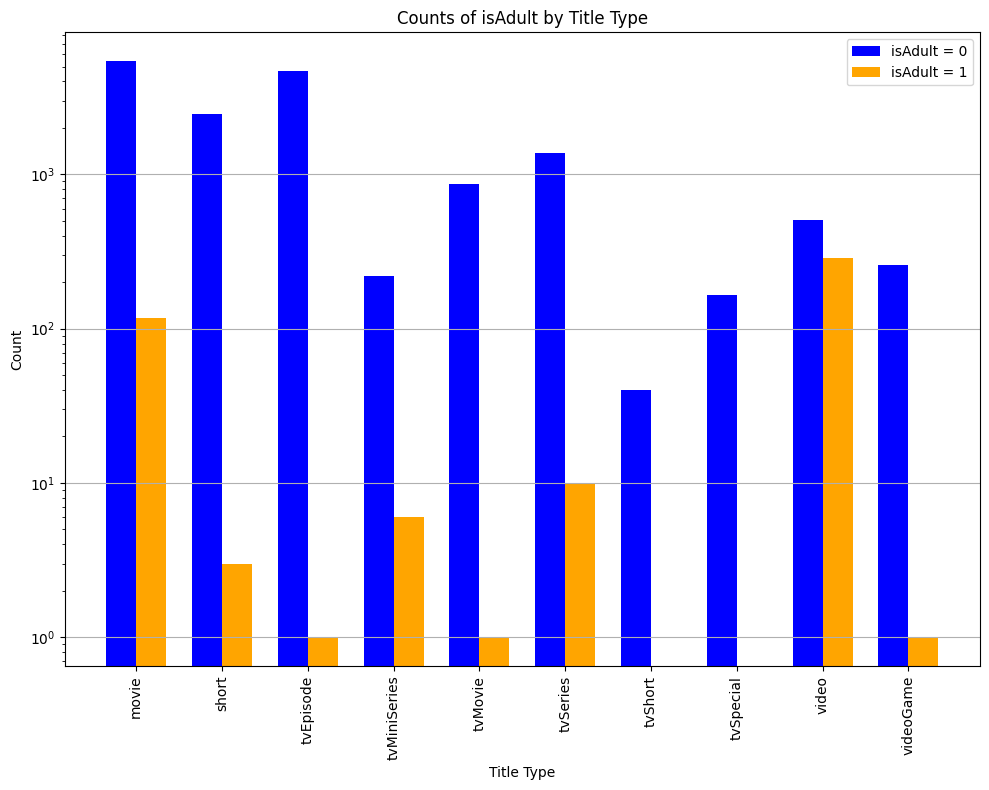
\includegraphics[width=0.48\textwidth]{plots/fig1_c.png}
%     }
%     \subfigure[]{
%         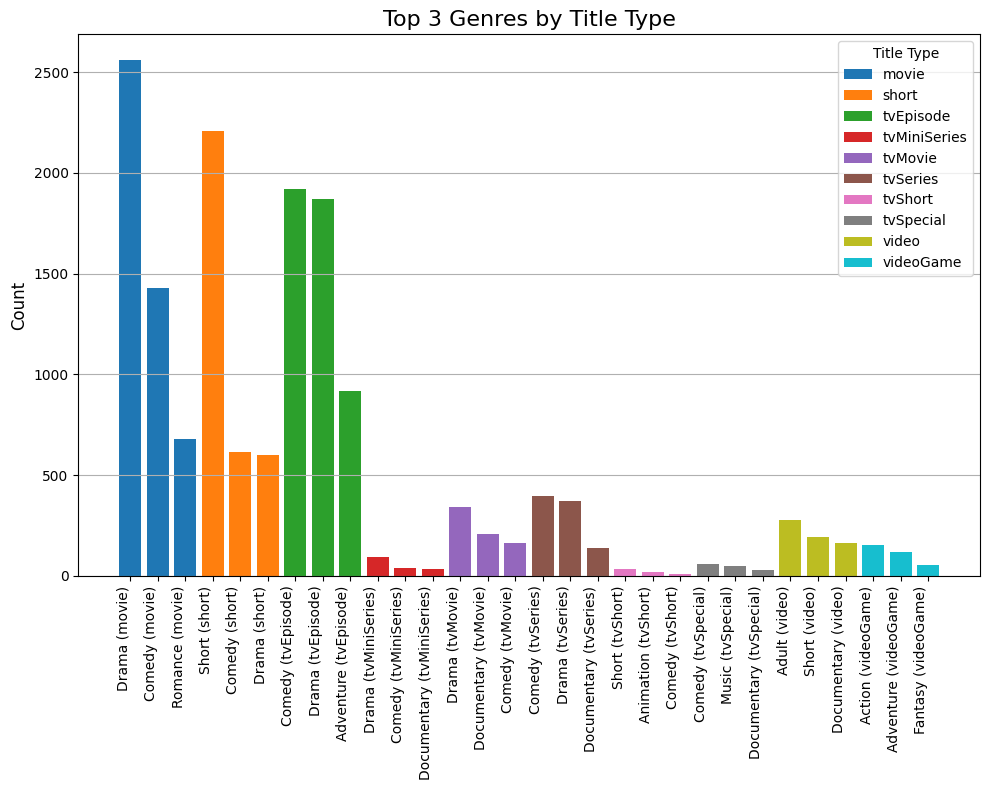
\includegraphics[width=0.48\textwidth]{plots/fig1_d.png} 
%     }
%     \caption{Bar chart of the discrete attributes
%     (b): counting of ratings frequencies;
%     (c): counting of the adult and non-adult frequencies combined with the
%     isRatable attribute;
%     (d) top 3 genres according to the titleType.}
%     \label{fig:bar-charts}
% \end{figure}


\begin{figure}[H]
    \centering
    % First subfigure
    \begin{subfigure}{0.48\textwidth}
        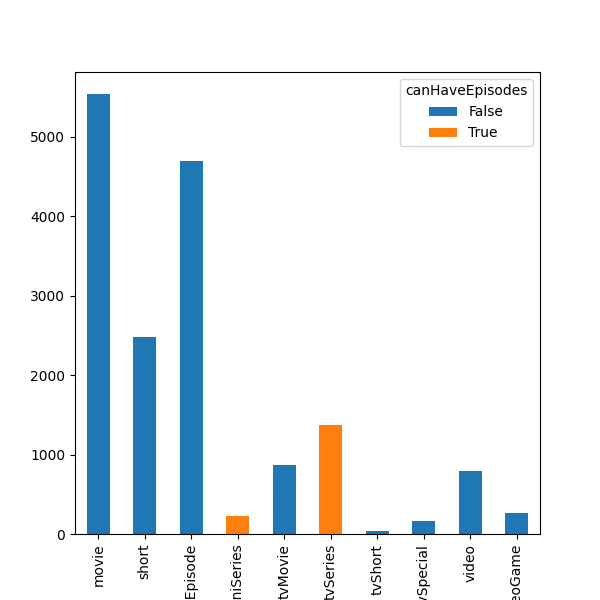
\includegraphics[width=\textwidth]{plots/fig1_a.png}
        \caption{Counting of the title types frequencies} %  combined with the canHaveEpisodes variable
        \label{fig:sub1}
    \end{subfigure}
    \hfill
    % Second subfigure
    \begin{subfigure}{0.48\textwidth}
        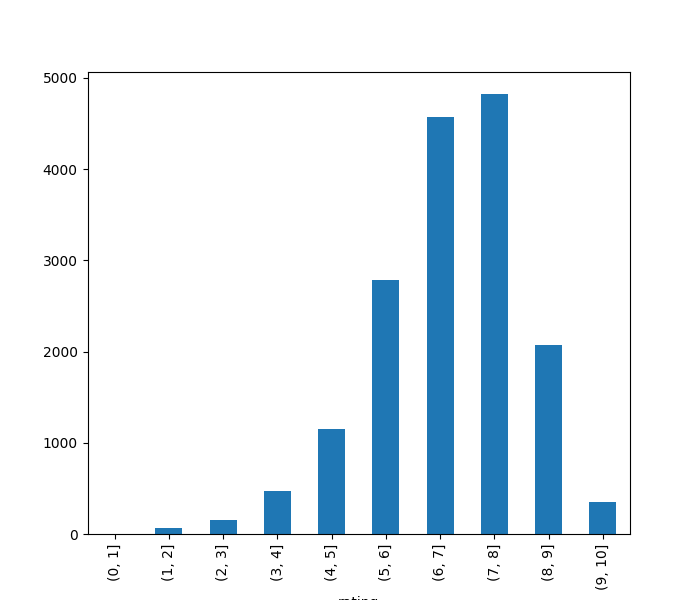
\includegraphics[width=\textwidth]{plots/fig1_b.png}
        \caption{Counting of ratings frequencies}
        \label{fig:sub2}
    \end{subfigure}
    
    % Third subfigure
    \begin{subfigure}{0.48\textwidth}
        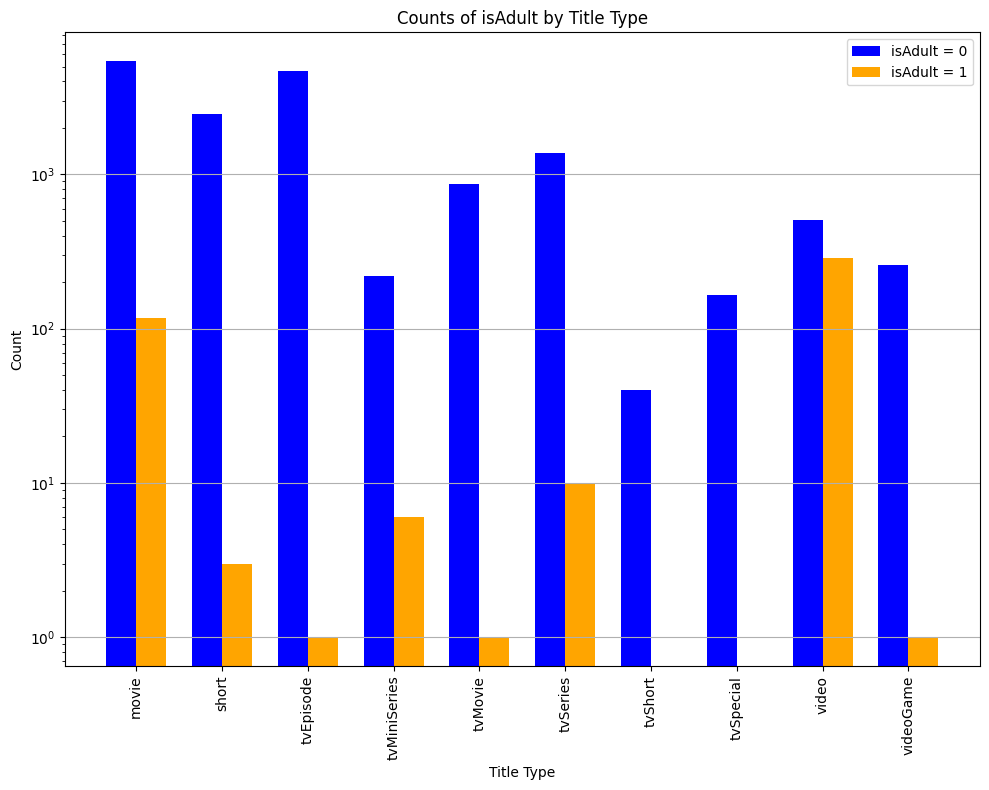
\includegraphics[width=\textwidth]{plots/fig1_c.png}
        \caption{Counting of the adult and non-adult per type}
        \label{fig:sub3}
    \end{subfigure}
    \hfill
    % Fourth subfigure
    \begin{subfigure}{0.48\textwidth}
        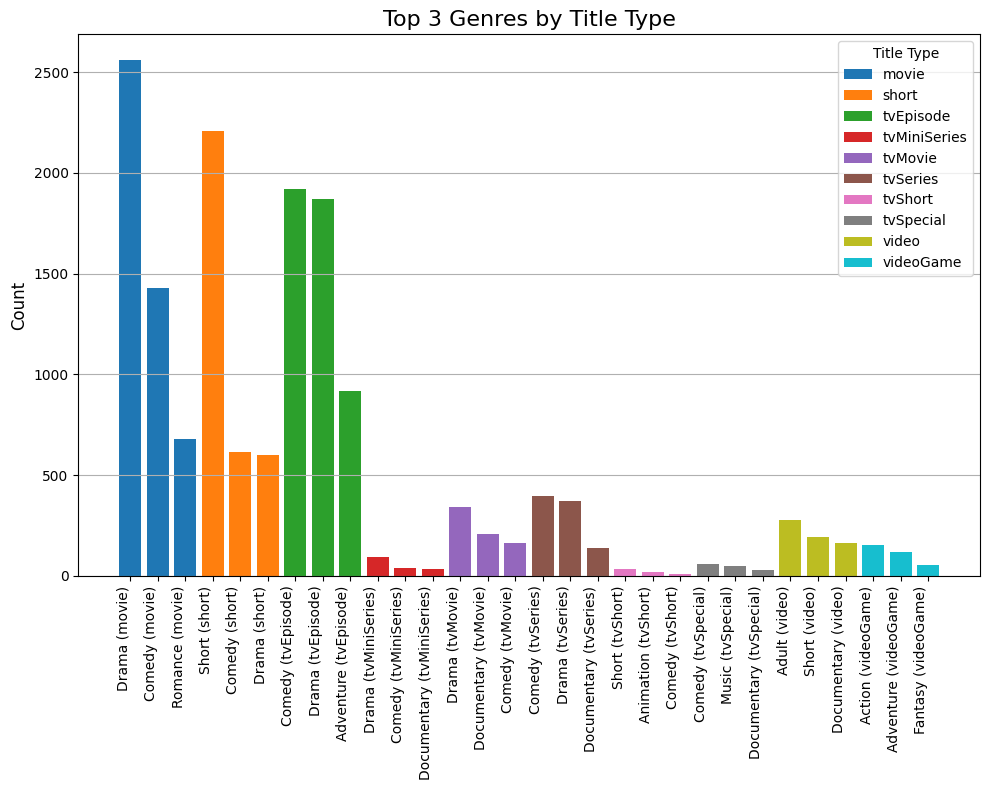
\includegraphics[width=\textwidth]{plots/fig1_d.png}
        \caption{types per genre}
        \label{fig:sub4}
    \end{subfigure}
    
    \caption{Bar chart of the discrete attributes.}
    \label{fig:bar-charts}
\end{figure}

\subsection{Continuous attributes}
...content...content...content...content...content...content...

\section{Data Quality}\label{sec:data_quality}
In this phase, a proper evaluation of the observed data was conducted in preparation for the analysis.
Once having checked that there are no duplicates and no incomplete rows in the dataset, attention was given at identifying missing values and outliers within the columns.

\subsection{Outliers detection}
While examining the dataset, it became apparent that some attributes have outliers. 
The important aspect to highlight is that since \texttt{awardWins}, \texttt{totalVideos} and \texttt{awardNominationsExcludeWins} have many values as 0 (respectively 14589, 14821, 14427), 
these might be considered variables with many outliers (as seen in Figure \textbf{METTERE GRAFICO che rappresenti in qualche modo il result di DETECT\_OULIERS\_MULTI\_ATTRIBUTES in data\_quality noemi}) but they actually have less outliers compared to the other variables.
For the other attributes \textbf{CONTINUARE......}


\subsection{Syntactic Inconsistencies}
In the exploration of the dataset it has been noticed that \texttt{awardWins} was the only feature having missing values identified with NaN.
However, there were missing values also in other columns (\texttt{endYear}, \texttt{runtimeMinutes} and \texttt{genres}), but they were indicated with the string "\textbackslash N".
To avoid this inconsistency causing problems during data preparation, these values have been replaced with NaN.
By doing so, any cell in the \texttt{endYear}, \texttt{runtimeMinutes} and \texttt{genres} column that previously contained the string "\textbackslash N" is now considered a proper missing value, detectable and manageable using Pandas' functions.

\subsection{Missing Values}
Once having solved the above-mentioned inconsistency, the resulting total amount of the missing values are the following, also represented in percentages for a better understanding:
\begin{itemize}
    \item \texttt{endYear}: it is the feature with the highest number of NaN values (15617; about 95\%). To handle them it has been decided to \textbf{COSA FARE?};
    
    \item \texttt{runtimeMinutes}: it has 4852 missing values (29.5\%) that have been handled by grouping the records by \texttt{titleType} and substituting the NaN value with the median of each group;
    
    \item \texttt{awardWins}: this feature has 2618 NaN values (about 16\%). Since the mode associated with this variable is 0, it has been decided to substitute the missing values with 0;

    \item \texttt{genres}: it is 382 missing values (2.3\%). Having dealt this variable with a multi-label one-hot encoding process (as will be described in the \textit{Variable Transformation} section), a vector of all zeros is assigned to record with missing genres values.
\end{itemize}

\section{Variable Transformation}\label{sec:var_Transformation}
As the first step in the variable transformation process, the \texttt{CountryOfOrigin} and \texttt{genres} variables (datatypes: strings) were converted into lists of strings to facilitate further analysis. 
This transformation was necessary because some records contain multiple genres or countries as values for these variables.
Multi-label one-hot encoding was applied to the \texttt{genres} column; each unique genre was represented as a binary feature, allowing records that belong to multiple genres simultaneously to maintain this information.
Furthermore, it has been decided to extract the ceiling value for each entry in the \texttt{rating} column, in order to use it as an integer for further analysis.\\

For the numeric attributes, it was observed that some variables required a stronger transformation due to their highly positively skewed distributions. 
Specifically, a log-transformation was applied to all the numeric attributes, since their skewness was highly greater than 1. 
This step was performed directly on the dataset. 
For the application of the different data mining techniques, \texttt{MinMaxScaler} and \texttt{StandardScaler} standard normalization techniques have been applied; respectively to scale each feature to a given range and to standardize features by removing the mean and scaling to unit variance.
The choice between these two methods was made based on the specific requirements of each data mining technique and the most suitable normalization approach for the task at hand.

\section{Pairwise correlations and elimination of variables}\label{sec:correlation}

The plot in figure~\ref{fig:correlation_matrix} is a Pearson's correlation matrix that takes into account the continuous numerical variables of the dataset.
For what can be observed, \texttt{numVotes} and \texttt{ratingCount} have a perfect positive correlation, and so it would be redundant to keep them both.
For this reason it has been decided to drop \texttt{ratingCount}. 
On the other hand, regarding categorial attributes, after having analized them, \texttt{bestRating}, \texttt{worstRating}, and \texttt{isRatable} have been discarded because they \textbf{endyear(???)} were found to have limited contribution based on their distributions.
As a matter of fact, their unique values were respectively 10, 1 and True for all attributes.
\begin{figure}[h!] % Positioning options: h (here), t (top), b (bottom), p (page)
    \centering % Centers the figure
    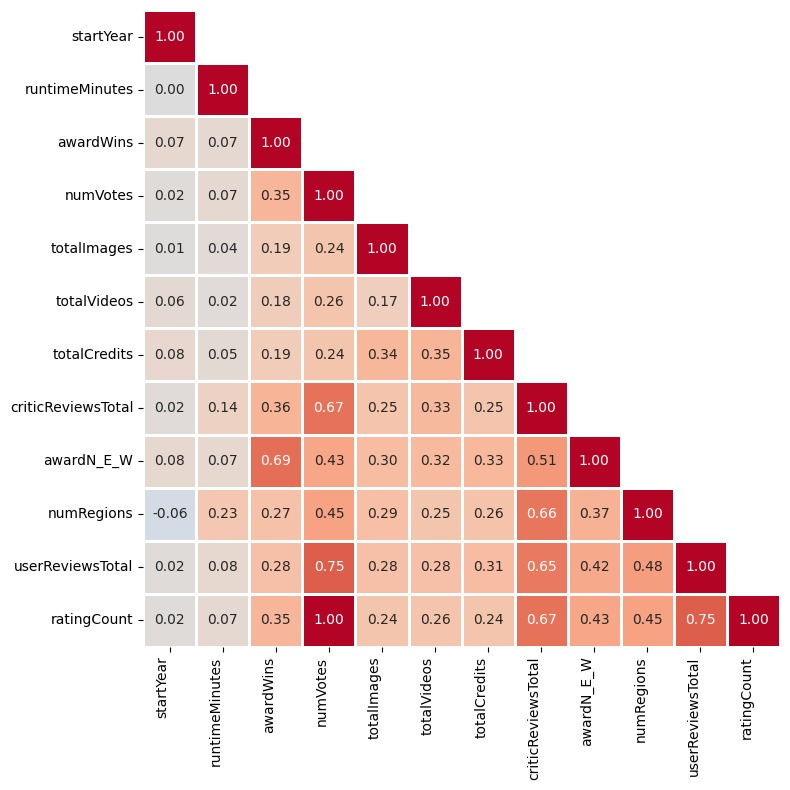
\includegraphics[width=0.8\textwidth]{plots/correlation_matrix.png} % Specify the file name and scaling options
    \caption{Correlation matrix} % Add a caption
    \label{fig:correlation_matrix} % Add a label for referencing
\end{figure}
